\documentclass[a4paper, 12pt]{article}
\usepackage{comment} % enables the use of multi-line comments (\ifx \fi)
\usepackage{fullpage} % changes the margin
\usepackage{enumitem}
\usepackage{graphicx}
\usepackage{hyperref}
\usepackage{wrapfig}


\begin{document}
%Header-Make sure you update this information!!!!
\noindent
\large\textbf{Visual Analytics - Final Project} \normalsize \hfill Due Date: 06/06/2018 \\
\normalsize Engineering in Computer Science   \\
Prof. Giuseppe Santucci \hfill Valerio Colitta - 1656690 \\
TA: Marco Angelini \hfill Davide Spallaccini - 1642557

\section*{Flights And Delays In The United States}

\paragraph{Introduction}
The airline industry is one of the fields that continuously produces a large amount of complex data
regarding the large number of flights that take place every day. In this work we concentrate only on
flights of a single year in the United States. Even considering a single nation and a single year the
number of flights is really high, so in this work we aim at providing a visualization of this data that
helps in better understanding patterns in the number of flights in the different states and in the 
delays that were recorded across time.

\paragraph*{Data}
We got our data from the United States Department of Transportation, and in particular from the 
Bureau of Transportation Statistics (BTS) website. As the independent statistical agency within the
Department of Transportation (DOT), the Bureau of Transportation Statistics (BTS) is a politically
objective supplier of trusted and statistically sound baseline, contextual, and trend information used
to shape transportation policy, investments, and research across the U.S. and abroad. BTS is the
preeminent source of statistics on commercial aviation, and transportation economics.
In particular we used the On-Time Performance table (available at ...) under the Airline and Airports
subsection of the website. This table contains on-time arrival data for non-stop domestic flights by
major air carriers, and provides such additional items as departure and arrival delays, origin and
destination airports, flight numbers, scheduled and actual departure and arrival times, cancelled or
diverted flights, taxi-out and taxi-in times, air time, and non-stop distance.
\\
\\
This dataset is very large and contains more than \texttt{5 millions} records of flights in the United
States just for 2017. 
The features we considered for the analysis and visualization will have the following symbols and
meanings:
\begin{itemize}
	\item \texttt{ARR\_DELAY} : minutes of delay on the arrival of the flight.
	\item \texttt{DEP\_DELAY} : minutes of delay on the departure of the flight.
	\item \texttt{AIR\_TIME} : minutes of air-time (duration of the flight).
\item \texttt{DISTANCE} : distance in miles covered by the airplane.
\item \texttt{CARRIER\_DELAY} : carrier delay in minutes.
\item \texttt{NAS\_DELAY}: National Air System delay, in minutes.
\item \texttt{LATE\_AIRCRAFT\_DELAY} : late aircraft delay in minutes.
\item \texttt{ORIGIN\_STATE\_ABR} : state of departure abbreviation.
\end{itemize}
Because of the considerable amount of data, we couldn't just load them via d3 or javascript; 
we tried, but the time to load it was just too much. Therefore we decided to do some preprocessing on
the data, before loading them.\\
Flights were grouped by \texttt{month, state} and counted to use those values in the \texttt{USA map}.
The same happened for the \texttt{DD scatter plot}\\ \\
In addition to that, we randomly sampled about a thousand records, in order to plot the single instances
on the parallel coordinates, and perform the PCA on them.

\paragraph*{State Patterns}
The first visualization elements we are going to describe have the goal to display for each state the 
amount of airline departures. In particular we want to visualize how many flights leave each state during
the different months of the year and how these numbers vary from state to state. For the first task we
drew a map of the USA and colored each state according to the number of flights for the selected month
with a heat map. The color of each state in this case is independent from the color of the other states,
it only depends on the mean of flights for that state during the year. A \emph{hot} color tells that in
that month the number of flights was higher than the average while a \emph{cold} color that the number of
flights was respectively low. A slider under the map allows the user to change the month under
consideration. On the other hand, in order to visualize how the number of flights differs from state to 
state in a quantitative fashion we display a bar chart with a bar for each state whose height is
proportional to the number flights in that state. When you click on a bar the bar becomes red and a line
appears cutting all the other bars at the height of the selected one, highlighting the differences; if 
then you over the mouse on other bars the difference number (positive or negative) is shown.

%% why map and why bar chart?

We found interesting that some patterns appear really clear in the map, for example in February almost
everywhere the number of flights is below the average, on the contrary in August this number is far over
the average probably highlighting the departures due to holidays. In July the same observations hold,
and in particular northern countries tend to have higher increase of flights. An exception to the summer 
excitement is Florida, probably because it is one of the destination for holiday travels and local
population usually stays in the country.\\
\begin{figure}[h]
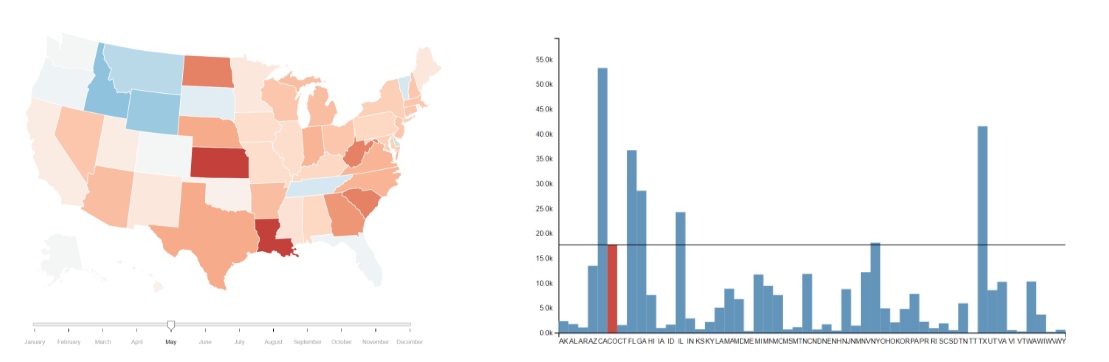
\includegraphics[scale=0.7]{usamapbar.PNG}
\end{figure}
\\

\paragraph*{Delays}
The other visualization elements we devised concern flights delays.
\\
This data is displayed in three views:
\begin{itemize}
\item A plot representing the results of a PCA projection of flights.
\item Parallel Coordinates with the attributes mentioned above.
\item A Distance-Delay scatter with some novel/peculiar characteristics.
\end{itemize}


\subparagraph{PCA plot} 
This plot displays in 2D the records sampled in the dataset projected along the attributes
with greater variance according to a PCA. We didn't plot the entire dataset but we picked uniformly
at random for each month a certain amount of data and used them for the visualization. Plotting all
the flights would have been too dense and it would have been difficult to distinguish points in the
plot. Moreover the size of the data would have required a considerable amount of computation time
on a Javascript engine and would have result in a bad delay experience for the user.
\\
Since we were concentrating on flights delays we selected only the flights that experienced some delay
at the arrival, at the departure or both.
\\
\begin{wrapfigure}{l}{0.54\textwidth}
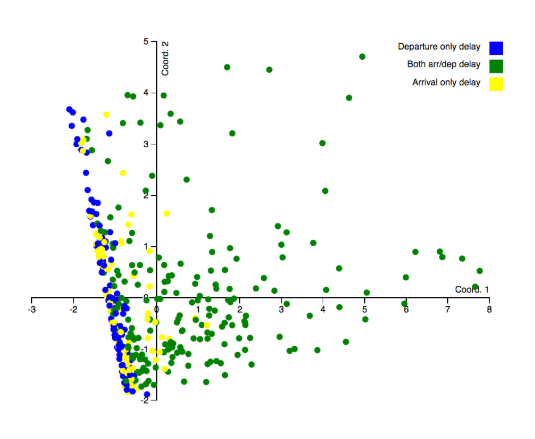
\includegraphics[scale=0.7]{pca.PNG}
\end{wrapfigure}
\\ 
Even if we didn't identify clusters after the data was projected we grouped the results according to
three different characteristics and we later observed on the plot thet they were actually close
together in the final space as you can see in the figure. So we divided the flights in three groups: the
ones that experienced a delay only during the departure, the ones that only arrived late, and the ones
that both leaved and arrived late.
\\
\\
As you can notice flights groups form clusters, and thus there is a good chance that
they are close each other also in higher dimensions.
\clearpage

\subparagraph{Parallel Coordinates}
The same data used in the PCA plot are displayed in all of their dimensions in a parallel coordinates
view. Paralle Coordinates are a standard method to visualize high-dimensional data on a 2D environment. 
As for the PCA plot we only displayed numerical features that concerned delays. Indeed for the dataset we
chose these were the only non-categorical values available.
\\
\begin{figure}[h]	
\centering
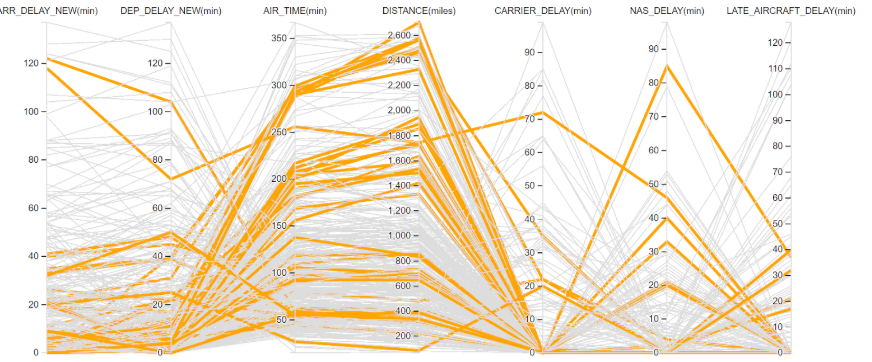
\includegraphics[scale=0.7]{pc.PNG}
\end{figure}\\
To give a better user-experience, axes can be moved around and reordered while maintaining a constant 
distance. To provide further user interaction in each of the axes the user can brush with the mouse over
an interval of values for that axis, as a results the lines in that interval are put in foreground and
the rest of the flights changes to a light grey color and is put in background.
\\
This view is also coordinated with the USA map. Indeed the user can click on a state and as a 
consequence in the parallel coordinated view only the flights that left that state are highlighted in an
orange color and put in foreground.

\subparagraph{Distance-Delay (DD) scatter} 
The last view in the second group is the DD scatter. It displays relationships between flight delays and
the distance of the origin and destination airports.
We decided to use a particular instance of a scatter plot where on the x-axis we have ranges of 
distances, while on the y-axis we have intervals for the delays. Each cell represents the 
\textit{number of flights whose distances and delays lie in those intervals}.


The color of each circle encodes such a number of flights for each point and allows to see quickly
for which ranges and intervals the number of flights is higher giving the user possibly interesting
insights.
\\ 
\\
\begin{figure}[h]	
\centering
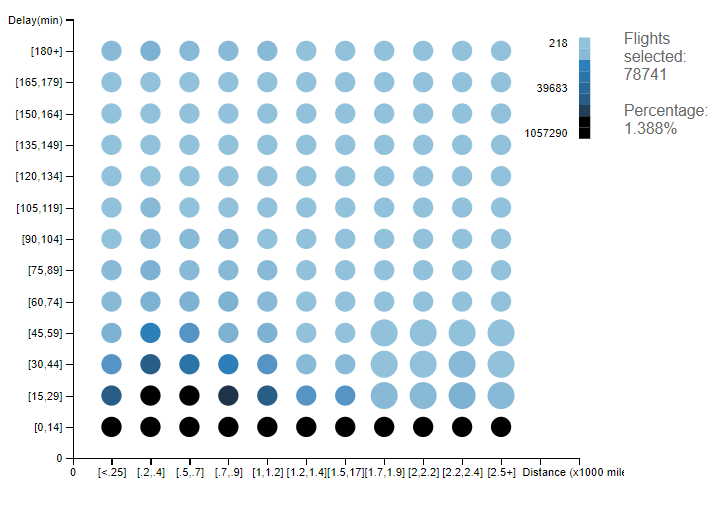
\includegraphics[scale=0.7]{ddscat.PNG}
\end{figure}
\\
Moreover, to give further details to the user, a group of points can be selected, and the exact number,
together with the percentage out of all flights the selection includes is displayed. This is useful in
order to "query" the dataset. For example, thanks to this view, we noticed that during the whole year of
2017, the number of flights that did not delayed more than 15 minutes is the 81\%, while those for which
the delay was greater than \texttt{3 hours} are only the 1\%, that is however about 60'000 flights.
\\
Other data extracted thanks to this view, is that most of the flights tend to cover about 500 - 1000
miles (as expected).
\\
\\
In the end we notice that the delays tend to decrease with the increase of the flight distance.
\paragraph{Why using this kind of plot?}
We opted for this over a correlation matrix for two main reasons. First, it works on two different
features and it is not symmetric, while usually a correlation matrix is symmetric.
\\
Second reason, we wanted it brushable, to have some interaction with it. In a correlation matrix this
would be possible, but in a less intuitive way.


\paragraph*{Conclusions}
In this work we devised a simple visual environment with the goal of displaying the number of flights 
and the entity of delays in the different states in the USA in a time interval of a year. We used a map
of the States coordinated with a bar chart to visualize across the various months the amounts of flights.
As for the delays we considered different numerical attributes of the flights especially regarding the
amounts of delay due to the possible different causes and displayed the data qualitatively in a PCA plot
and in the details in a parallel coordinates view. Finally we devised a novel scatter plot with colored
points in order to visualize the correlation between the distance of the origin and destination airports
and the total amount of delay.

As for future work we think it may be useful to add ...

(Slides for this project are available 
\href{https://docs.google.com/presentation/d/1T_p1oarqUuNt5APTaf7IwTJEzUDJC0CoNfJKHdak0so/edit?usp=sharing}{here}).


\end{document}
